


\paragraph{- Relative Time Protocol}



The elected validators for a slot need to know  when actually the right time to produce a block for the consistency and the security of the block production mechanism. For this purpose, they run the relative time protocol. This protocol depends on the arrival time of blocks according to local clocks of validators. Thus, it is named as ``Relative Time''.


In BABE, we assume that after the genesis block is released, elected validators of the first epoch store the arrival time of the genesis block with respect to their local clock. Then, they mark the start time of the first slot and increment the slot number every $ T $ seconds. After this point,  they periodically run the relative algorithm not to lose the synchronization with others because of their local clock drift.  In addition to this, a validator joins after the genesis block runs the relative time algorithm for synchronize with the other validators. Validators are synchronized if they have the same slot number in at least one moment in the original interval (Rephrase IT).


Assume that we have a validator who is a slot leader of the slot number $ \slot $ and  he wants to learn when $ \slot $ starts according to his local clock.  For this, he first collects $ n $ blocks. During the collection period, he stores  the arrival time $ t_i $ of the block together with the slot number $\slot'_i$ in the block. Then, the validator computes some candidate start times of $ \slot $ using the arrival times and the slot numbers i.e,  given that $ \delta_i = T(\slot - \slot'_i)  $,  $\mathcal{C}_T = \{t_i+\delta_i \}_{1 \leq i \leq n} $. The times in $ \mathcal{C}_T $ is considered as candidates because of the following reason: We just for a moment imagine that  all  blocks are sent by honest and synchronized validators without any network delay. Given this fact, we say that $ \slot $ should start $ T(\slot - \slot'_i) $ seconds later. Therefore, all times are some candidates. In order to  choose one candidate,  the validator then sorts the list of candidates $ \mathcal{C}_T $ and outputs the median of the sorted list as a start time of the $ \slot $. An example execution of the relative time protocol is in Figure \ref{fig:relativetime}.

\begin{figure}[h]
	\centering
	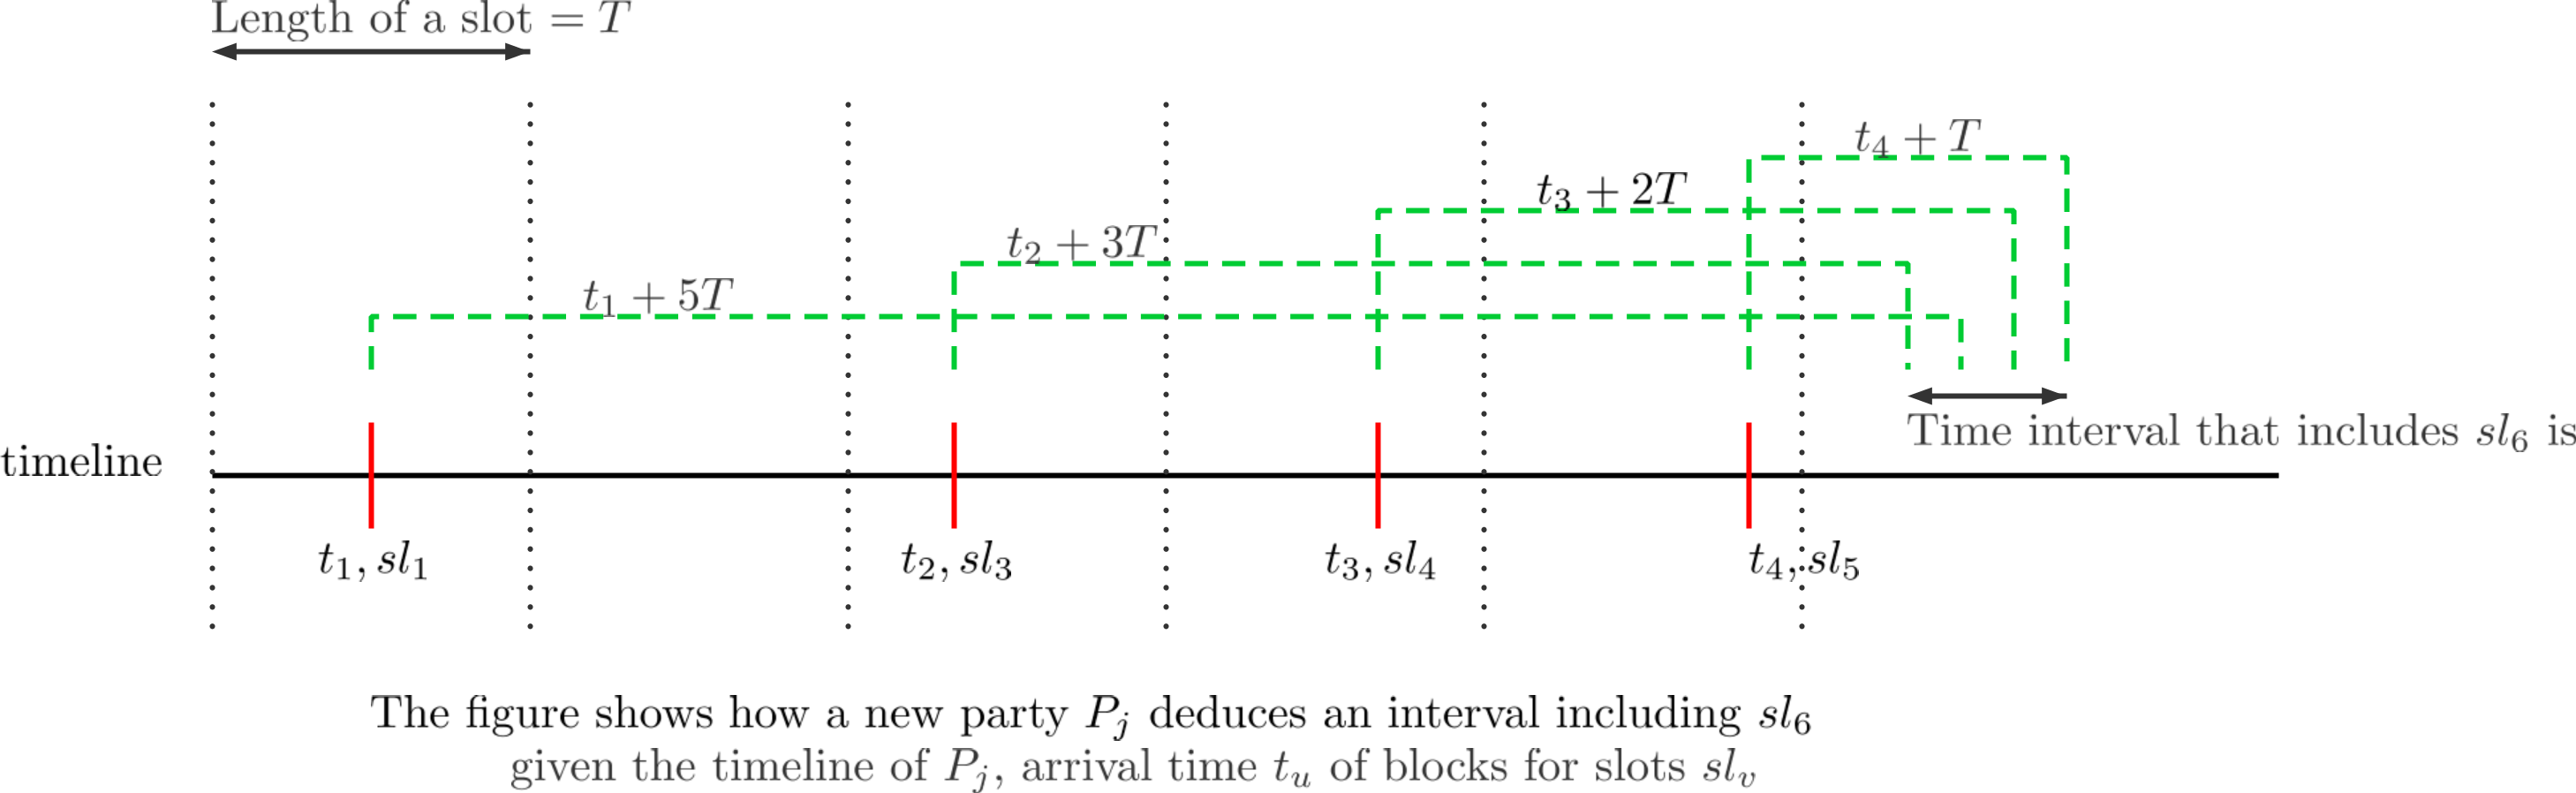
\includegraphics[width=1.\textwidth]{images/relative.png}
	\caption{An example execution of the relative time protocol by a validator who wants to learn $ \slot_{6} $.}
	\label{fig:relativetime}
\end{figure}



The relative time protocol guarantees that the output of a validator can be at most $ \D $ behind the slot number from the real slot number on assuming that at least half of the blocks during the collection period belong to honest and synchronized parties. The reason of this result based on the fact that half of $ n $ blocks belong to honest and synchronized validators with a very high probability. If the median is computed from an arrival time of block belonging to a honest and synchronized validator.